% Created 2020-12-15 二 22:04
% Intended LaTeX compiler: xelatex
\documentclass[11pt]{report}
\usepackage{graphicx}
\usepackage{grffile}
\usepackage{longtable}
\usepackage{wrapfig}
\usepackage{rotating}
\usepackage[normalem]{ulem}
\usepackage{amsmath}
\usepackage{textcomp}
\usepackage{amssymb}
\usepackage{capt-of}
\usepackage{hyperref}
\author{曹嘉祺 PB18030874 化学与材料科学学院 有机化学系 \thanks{中国 安徽合肥 中国科学技术大学 Email: \href{mailto:mkq@mail.ustc.edu.cn}{mkq@mail.ustc.edu.cn}}}
\usepackage[scheme=plain]{ctex}
\usepackage{fontspec}
\setmainfont{更纱黑体 UI SC}
\hypersetup{colorlinks=true,linkcolor=blue}
\usepackage{longtable}
\date{\today}
\title{液体饱和蒸汽压的测定}
\hypersetup{
 pdfauthor={曹嘉祺 PB18030874 化学与材料科学学院 有机化学系},
 pdftitle={液体饱和蒸汽压的测定},
 pdfkeywords={},
 pdfsubject={},
 pdfcreator={Emacs 27.1 (Org mode 9.4)}, 
 pdflang={English}}
\begin{document}

\maketitle
\tableofcontents

\begin{abstract}
本实验学习了液体的饱和蒸汽压、摩尔汽化热的概念,液体饱和蒸汽压与温度的关系,
以及动态法测定液体饱和蒸气压的基本原理和方法。通过测量在不同外压下的沸点,
就测得了液体的饱和蒸汽压,进而根据克拉贝龙-克劳修斯方程,
利用作图法进行直线拟合得出直线的斜率,并计算出液体的平均摩尔汽化热。


\noindent\rule{\textwidth}{0.5pt}
\begin{itemize}
\item 关键词: 饱和蒸汽压\quad 摩尔汽化热\quad 克拉贝龙-克劳修斯方程\quad 动态法
\end{itemize}
\end{abstract}
\begin{abstract}
In this experiment, we learn the concept of the saturated vapor pressure of the liquid,
the molar heat of vaporization, relationships of liquid saturated vapor pressure and temperature,
and the basic principles and methods of dynamic method of measurement of liquid saturation vapor pressure.
By measuring the boiling point in different boiling liquid, the saturated vapor pressure of the liquid had measured.
Then according to the Clausius-Clapeyron equation, using the mapping method for fitting a straight line,
the slope of the line is obtained, and calculating the average molar heat of vaporization of the liquid.

\noindent\rule{\textwidth}{0.5pt}

\begin{itemize}
\item key words:  Saturated vapor pressure, Molar heat of vaporization, Clapeyron-Clausius equation, Dynamic method
\end{itemize}
\end{abstract}
\part{前言}
\label{sec:orgb6570ec}
\chapter{实验原理}
\label{sec:org03f6aee}
\section{饱和蒸汽压、摩尔汽化热及克拉贝龙-克劳修斯方程}
\label{sec:org5433076}
在封闭体系中,液体很快和它的蒸汽达到平衡。这时的蒸汽的压力称为液体的饱和蒸汽压。蒸发一摩尔液体需要吸收的热量,即为该温度下液体的摩尔汽化热。
它们的关系可用克拉贝龙-克劳修斯方程表示:
\[
    \frac{d \ln p}{d T}=\frac{\Delta_{vap}H_{m}}{RT^{2}}
    \]
\begin{itemize}
\item \(\Delta\) H:摩尔汽化热(J\(\cdot\) mol\textsuperscript{-1})
\item R:气体常数(8.314J\(\cdot\) mol\textsuperscript{-1}\(\cdot\) K\textsuperscript{-1})
\end{itemize}
若温度改变的区间不大,H可视为为常数(实际上H与温度有关)。积分上式得:
\[
    \ln P = A'-\frac{\Delta H}{RT}
    \]
或:
\[
    \log P = A-\frac{B}{T}
    \]
其中\(A=\frac{A'}{2.303}\) ,\(B=\frac{\Delta_{vap}H_{m}}{2.303R}\) 上式表明\(\log P\) 与\(\frac{1}{T}\) 有线性关系。
作图可得一直线,斜率为\(B\) 。因此可得实验温度范围内液体的平均摩尔汽化热\(\Delta H\) 。
\[
    \Delta_{vap}H_{m}=2.303 R B
    \]
\section{不同外压下液体的沸点的测量方法}
\label{sec:org08b5f4c}
当外压为\(101.325kPa(760mmHg)\) 时,
液体的蒸汽压与外压相等时的温度称为液体的正常沸点。在图上,也可以求出液体的正常沸点。

液体饱和蒸汽压的测量方法主要有三种:
\begin{itemize}
\item 静态法:在某一固定温度下直接测量饱和蒸汽的压力。
\item 动态法:在不同外部压力下测定液体的沸点。
\item 饱和气流法:在液体表面上通过干燥的气流,调节气流速度,使之能被液体的蒸汽所饱和,然后进行气体分析,计算液体的蒸汽压。
\end{itemize}

本实验利用第二种方法。此法基于在沸点时液体的饱和蒸汽压与外压达到平衡。只要测得在不同外压下的沸点,也就测得在这一温度下的饱和蒸汽压。

\part{实验部分}
\label{sec:org2c506ac}
\chapter{实验仪器与试剂}
\label{sec:org0d63eb9}
\section{仪器}
\label{sec:org8be506e}
\begin{table}[htbp]
\caption{实验仪器}
\centering
\begin{tabular}{lll}
仪器 & 数目 & 厂家\\
\hline
数字式低真空测压计 & 1套 & 南京南大万和科技有限公司\\
真空泵 & 1台 & 郑州长城科工贸有限公司\\
U形压力计 & 1支 & 江苏省常州市东风仪表厂\\
电动搅拌器 & 1台 & 金坛市环宇科学仪器厂\\
DTC-2AL控温仪 & 1台 & 南京南大万和科技有限公司\\
真空稳压包WYB-I & 2台 & 南京南大万和科技有限公司\\
\end{tabular}
\end{table}

\chapter{装置简介}
\label{sec:org4bd73a0}
下图中,平衡管由三个相连通的玻璃球构成,顶部与冷凝管相连。
冷凝管与U形压力计6和缓冲瓶7相接。
在缓冲瓶7和安全瓶11之间,接一活塞9,用来调节测量体系的压力。
安全瓶中的负压通过真空泵抽真空来实现。安全瓶和真空泵之间有一三通阀,
通过它可以正确地操作真空泵的启动和关闭。A球中装待测液体,当A球的液面上纯粹是待测液体的蒸汽,
并且当B管与C管的液面处于同一水平时,
表示B管液面上的蒸汽压(即A球面上的蒸汽压)与加在C管液面上的外压相等。
此时体系汽液两相平衡的温度称为液体在此外压下的沸点。
用当时读得的大气压减去压差计两水银柱的高度差,即为该温度下液体的饱和蒸汽压。

\begin{figure}[htbp]
\centering
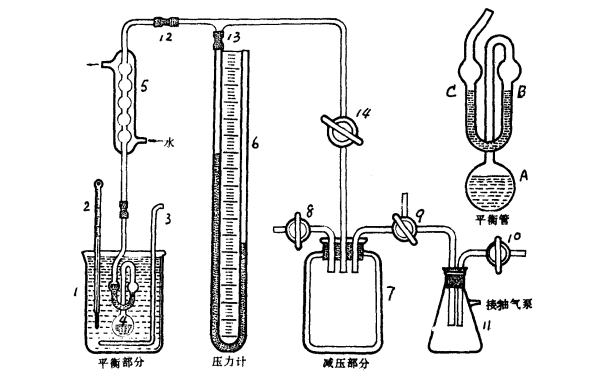
\includegraphics[width=.9\linewidth]{../img/1.png}
\caption{纯液体饱和蒸汽压测定装置图}
\end{figure}

\begin{enumerate}
\item 盛水大烧杯;
\item 温度计(分度值为0.1\textsuperscript{o}C);
\item 搅拌;
\item 平衡管;
\item 冷凝管;
\item 开口U形水银压力计;
\item 具有保护罩的缓冲瓶;
\item 进气活塞;
\item 抽气活塞;
\item 放空活塞;
\item 安全瓶;
\item 橡皮管;
\item 橡皮管;
\item 三通活塞;
\end{enumerate}

其中1、2、3、4、5组成了恒温水浴系统,用于恒温;6、7等组成了压力测量系统,
用以测量不同温度下的压力差;11、水泵组成了辅助系统,用以提供真空。

\begin{itemize}
\item 注: 其中安全瓶用减压包代替,温度计改为数显
\end{itemize}

\chapter{实验步骤}
\label{sec:org8059aa3}
\section{熟悉实验装置}
\label{sec:org0425331}
掌握真空泵的正确使用,了解系统各部分及活塞的作用,读当日大气压(整个实验过程中要读取3次)。
\section{装样}
\label{sec:org24a698b}
取下平衡管4,洗净、烘干,装入待测液。使A球内有2/3体积的液体。
并在B,C管中也加入适量液体,将平衡管接在冷凝管的下端。

平衡管中液体的装法有两种:
\begin{itemize}
\item 把A管烘烤,赶走空气,迅速在C管中加入液体,冷却A管,把液体吸入。
\item 将C管中加入液体,将平衡管与一水泵相连接,抽气,并突然与水泵断开,让C管的水流入A管。

\item 注:实验时并未进行平衡管中的装液操作,液体已事先装好
\end{itemize}
\section{系统检漏}
\label{sec:org528ce93}
关闭活塞8和9,将三通活塞14旋转至与大气相通,关闭活塞10,插上真空泵电源,启动真空泵,将活塞14再转至与安全瓶11相通,抽气5分钟,再将活塞14旋至与大气相通,拔掉真空泵电源,停止抽气。这样做是为了防止真空泵油倒吸。(注:实验中泵一直未关闭)用活塞9调节缓冲瓶的真空度,使U形压力计两臂水银柱高低差为20—40毫米,关闭活塞9。仔细观察压力计两臂的高度,
在10分钟内不变化,证明不漏气,可开始做实验。否则应该认真检查各接口,直到不漏气为止。

\begin{itemize}
\item 注: 实验时并未检漏或检漏工作已经由老师提前完成
\end{itemize}
\section{不同温度下液体饱和蒸汽压的测定}
\label{sec:org7231b12}
\begin{enumerate}
\item 组装仪器
\label{sec:org049d710}
将平衡管浸入盛有蒸馏水的大烧杯中,并使其全部浸没在液体中。插上电炉加热,同时开冷却水,
开启搅拌马达,使水浴中的水温度均匀。
\begin{itemize}
\item 注: 由老师完成
\end{itemize}
\item 将稳压包抽真空
\label{sec:orgd45eb66}
关闭活塞9,使活塞8与大气相通。此时平衡管,压力计,缓冲瓶处于开放状态。将活塞14通大气,插真空泵电源抽气,
把活塞14旋转至与安全瓶相通,抽5分钟,再将活塞14通大气。拔下电源,此时安全瓶内为负压,待用。
\begin{itemize}
\item 注: 这里的安全瓶指与泵直接相连的稳压包
\end{itemize}
\item 测大气压下液体的沸点
\label{sec:org4b4dee3}
随着水浴中液体的温度的不断升高,A球上面的待测液体的蒸汽压逐渐增加,使C管中逐渐有气泡逸出。
本实验所测的液体为环己烷,待测水浴中的液体沸腾后仍需继续煮沸5-10分钟,
把A球中的空气充分赶净,使待测液上面全部为纯液体的蒸汽。停止加热,让水浴温度在搅拌中缓缓下降,
C管中的气泡逐渐减少直至消失,液面开始下降,B管液面开始上升,认真注视两管液面,一旦处于同一水平,
立即读取此时的温度。这个温度便是实验大气压条件下液体的沸点。
\item 测不同外压下液体的沸点
\label{sec:org56d27ec}
关闭活塞8,用活塞9调节缓冲瓶7中的真空度,从而降低平衡管上端的外压,
U形压力计两水银柱相差约40mm左右,这时A管中的待测液又开始沸腾,C管中的液面高于B管的液面,并有气泡很快逸出,随着温度的不断下降,气泡慢慢消失,B管液面慢慢升高,在B、C两管液面相平时,说明A、B之间的蒸汽压与外压相等。立即记下此时的温度和数字压力计上的读数。此时的温度即外压为大气压减去压力计压强的情况下液体的沸点。

继续用活塞9调节缓冲瓶的压力,体系产生新的沸腾,再次测量蒸汽压与外压平衡时的温度,反复多次,约10个点。温度控制在80C以上,压差计的水银柱相差约400mm左右为止。

为了测量的准确性,可将缓冲瓶放空,重新加热,按上述步骤继续重复测量两次。

实验结束时,再读取大气压,把两次记录的值取平均。(实际操作时实验中也测了一次大气压,所以是三次平均)
\item 校准数字压力计
\label{sec:orgd5d6df2}
在上一个步骤中, 选择一次将U形管的读数和数字压力计的读数同时读出,记录
\end{enumerate}

\chapter{实验数据及数据处理(见附件)}
\label{sec:org56b5e58}
\chapter{结果分析与讨论}
\label{sec:orgc09fc53}
\section{实验结果}
\label{sec:org2e93902}
\begin{enumerate}
\item 摩尔汽化热
\label{sec:org60a1960}
三次实验得到的摩尔汽化焓分别为:
\[
    \Delta_{vap}H_{m1}=RB=8.314\times 3834.6=31880.864(J\cdot mol^{-1})
    \]
\[
    \Delta_{vap}H_{m2}=RB=8.314\times 3735.18=31054.287(J\cdot mol^{-1})
    \]
\[
    \Delta_{vap}H_{m3}=RB=8.314\times 3883.25=32285.341(J\cdot mol^{-1})
    \]
均值计算:
\[
    \overline{\Delta_{vap}H_{m}}=\frac{\Delta_{vap}H_{m1}+\Delta_{vap}H_{m2}+\Delta_{vap}H_{m3}}{3}
    \]
\[
    \overline{\Delta_{vap}H_{m}}=(31880.864+31054.287+32285.341)/3=31740.164(J\cdot mol^{-1})
    \]
经百度得知环己烷的摩尔汽化热为31.51 kJ/mol(不同资料给出的结果不同),所以两者的相对误差为:
\[
    w=\frac{31740.164-31510}{31510}\times 100\% =0.73\%
    \]
由上述相对误差可知,实验所测的平均摩尔汽化热与理论摩尔汽化热相差较小,说明实验结果的准确性。
\item 沸点计算
\label{sec:org8811b4b}
\begin{enumerate}
\item 第一组(353.49(K))
\label{sec:org633cd71}
拟合曲线为:
\[
     \ln(p)=-\frac{3834.6}{T}+22.3739
     \]
所以当压力为大气压即P=101325Pa时,温度即沸点为:
\[
     T=-\frac{3834.6}{\ln(101325)-22.3739}=353.49(K)
     \]
\item 第二组(353.93(K))
\label{sec:orgc8adf8e}
拟合曲线为:
\[
     \ln(p)=-\frac{3735.18}{T}+22.0794
     \]
所以当压力为大气压即P=101325Pa时,温度即沸点为:
\[
     T=-\frac{3735.18}{\ln(101325)-22.0794}=353.93(K)
     \]
\item 第三组(353.42(K))
\label{sec:org8ebfafc}
拟合曲线为:
\[
     \ln(p)=-\frac{3883.25}{T}+22.5136
     \]
所以当压力为大气压即P=101325Pa时,温度即沸点为:
\[
     T=-\frac{3883.25}{\ln(101325)-22.5136}=353.42(K)
     \]
\item 误差分析
\label{sec:org5e56687}
查得(经百度百科)环己烷在大气压下的理论沸点为80.7\textsuperscript{o}C,即353.85K,与实验所测的沸点进行比较可知,
绝对误差及相对误差分别为:
\begin{enumerate}
\item 第一组
\label{sec:orge79bf48}
\[
      \Delta T=353.49-353.85=-0.36(K)
      \]
\[
      w=\frac{|\Delta T|}{T}=\frac{0.36}{353.85}=0.10\%
      \]
\item 第二组
\label{sec:org5a92db1}
\[
      \Delta T=353.93-353.85=0.08(K)
      \]
\[
      w=\frac{|\Delta T|}{T}=\frac{0.08}{353.85}=0.02\%
      \]
\item 第三组
\label{sec:orgab98356}
\[
      \Delta T=353.42-353.85=0.43(K)
      \]
\[
      w=\frac{|\Delta T|}{T}=\frac{0.43}{353.85}=0.12\%
      \]
\item 结论
\label{sec:orgea64bf2}
由上述相对误差可知,实验所测的正常沸点与理论值偏差较小,
说明实验结果较为准确,实验方法较为合理。
\end{enumerate}
\end{enumerate}
\end{enumerate}

\section{实验讨论}
\label{sec:org74e747f}
\begin{enumerate}
\item 误差分析
\label{sec:org2c85bc7}
影响测量准确度的因素如下:
\begin{enumerate}
\item 恒温水浴的温度不均匀,可能是由于搅拌器搅拌速率太小或者是冷凝水通的速度过快导致水浴的温度来不及混匀。解决办法是加大搅拌器的搅拌速度,使搅拌更给力,或者减小冷凝水的速度并采取时开时关的策略,在降温初始打开,两液面快相平时关掉。
\item 系统有可能漏气,影响体系的真空度,并在测量时压差不断变化而影响测量,解决办法是如实验中操作的那样检漏。
\item 实验中由于采取的是动态法,判断平衡管B、C管液面相平很困难,管上也无法加刻度,只能目测,这样会带来较大的主观误差,目前还没有较好的解决办法。
\item 为了防止水银的挥发,在U形压力计上端加了水进行液封,但是这样做,当两管中的液面不平时由于U形压力计两侧管的内径不同,两侧的液面上升和下降的高度就会不同,在记录高度差时就要综合考虑水和水银的高度差,但由于水银的密度远大于水,在记录时可以忽略水的高度差带来的影响
\item 体系中的空气可能无法排净,这带来一定的误差,若混有空气等惰性气体时测得的饱和蒸汽压会偏高,即沸点可能偏高,解决办法是加热煮沸液体5\textasciitilde{}10min即可。另外,若测量中未来得及减压而使气体又进入A管,则需重新进行排气。
\item 平衡管巧妙之处在于A管中体系(液体和气体)的总体积不变,且体积小易被气体饱和,B—C之间的U形状液体所起到的主要作用是油封和指示压差。但是也存在一些缺点,如温度计无法放入平衡管去测量体系(液体和气体)的温度,测量的是恒温水浴的温度,解决的办法是在平衡管周围多加几个温度计或直接放进A管中测量;在测量完一个温度下的沸点后若不及时减压,则会容易产生倒吸,使外部气体又进入体系,或者使B—C之间的U形状液体进入体系,这会带来较大的误差。
\item 克拉伯龙-克劳修斯方程是建立在多个条件之上的,如:将蒸汽视为理想气体,在汽化过程前后忽略液体的体积,且在一定温度范围内认为摩尔汽化热为常数。而理想气体仅是理想化的模型,汽化过程之前的液体也占据一定的体积,而且摩尔汽化热实际上是随温度变化而变化的。虽然摩尔汽化热随温度变化不大,但是实验前后温差也不可过大,由实验中的数据记录可以发现,前后温差将近有20℃,这无疑会带来一定的误差,不过由作出的ln(P)-1/T关系曲线的线性可知,R\textsuperscript{2}均在0.9左右,说明直线的线性很好,在实验温度区间内摩尔汽化热基本不变。
\item 实验中是测量温度不断下降时的饱和蒸汽压,在测量时温度不断下降,而且下降速度较快,这就给温度的读数带来了一定的困难,会带来较大的读数误差,另外由于温度下降较快,很有可能体系的温度并不均匀;另一方面U形压力计两侧管的读数也会带来一定的误差,因为实验中是提前读的示数,且有时示数可能抖动,不太容易读准。
\end{enumerate}

\item 实验总结
\label{sec:org7694708}
本实验利用动态法测定了环己烷在不同温度下的饱和蒸汽压(或者是不同外压下的沸点),并利用克拉贝龙-克劳修斯方程,通过线性拟合的办法,求出了在实验温度下环己烷的摩尔汽化热及正常沸点,得出了与理论值相差很小的实验结果,说明了克拉贝龙-克劳修斯方程的准确性及实验方法的合理性。
\end{enumerate}
\part{参考文献}
\label{sec:org7f0381d}
\begin{enumerate}
\item 崔献英,柯燕雄,单绍纯.物理化学实验[M].合肥:中国科学技术大学出版社,2000.4
\item 傅献彩,沈文霞,姚天扬.物理化学.第四版.北京:高等教育出版社,1990.10
\item 杜达志等. 液体饱和蒸汽压的测定实验数据处理.江西:江西师范大学学报(自然科学版),1992.5.
\item 李震. 氧弹式量热法测燃烧热实验的改进.大学化学,2001.8
\item 百度百科数据库.
\item 李惠云,郭金福,栗鸿斌,郝存江. 简易动态法测定液体饱和蒸气压的装置.河南:大学化学,1998.10
\end{enumerate}

\part{附录: 数据处理过程}
\label{sec:org7c5c212}
\chapter{原始数据}
\label{sec:orgb3bddc8}
\section{大气压强}
\label{sec:org9e3fadc}
\begin{table}[htbp]
\caption{实验各时间段测定的大气压强}
\centering
\begin{tabular}{rr}
序号 & 压强(kPa)\\
\hline
1 & 102.98\\
2 & 102.94\\
3 & 102.92\\
4 & 102.99\\
average & 102.958\\
 & \\
\end{tabular}
\end{table}
\section{常压下液体的沸点}
\label{sec:org352c2e2}
\begin{table}[htbp]
\caption{常压下液体的沸点}
\centering
\begin{tabular}{rr}
序号 & 温度(\textsuperscript{o}C)\\
\hline
1 & 80.858\\
2 & 80.833\\
3 & 80.857\\
\end{tabular}
\end{table}

\section{不同外压下的沸点}
\label{sec:orge6ea5d4}
\begin{enumerate}
\item 第一组
\label{sec:org45804a0}
\begin{table}[htbp]
\caption{First}
\centering
\begin{tabular}{rrr}
序号 & 压强计(mmHg) & 温度(\textsuperscript{o}C)\\
\hline
1 & -33.9 & 79.463\\
2 & -70.4 & 77.789\\
3 & -115.2 & 75.631\\
4 & -155.3 & 73.606\\
5 & -195.3 & 71.458\\
6 & -234.6 & 69.242\\
7 & -273.2 & 66.935\\
8 & -312.8 & 64.400\\
9 & -351.4 & 61.768\\
10 & -390.1 & 58.928\\
\end{tabular}
\end{table}

\item 第二组
\label{sec:org8510fb3}
\begin{table}[htbp]
\caption{Second}
\centering
\begin{tabular}{rrr}
序号 & 压强计(mmHg) & 温度(\textsuperscript{o}C)\\
\hline
1 & -386.4 & 59.192\\
2 & -352.6 & 61.676\\
3 & -313.9 & 64.329\\
4 & -274.6 & 66.846\\
5 & -236.3 & 69.154\\
6 & -198.8 & 71.279\\
7 & -157.4 & 73.507\\
8 & -120.6 & 75.386\\
9 & -81.3 & 77.308\\
10 & -42.2 & 79.134\\
\end{tabular}
\end{table}

\item 第三组(校准)
\label{sec:orgde49c6c}
\begin{table}[htbp]
\caption{Third}
\centering
\begin{tabular}{rrrrrr}
序号 & 压强计(mmHg) & U管左(cm) & U管右(cm) & 高度差(mmHg) & 温度(\textsuperscript{o}C)\\
\hline
1 & -36.9 & -1.80 & 1.98 & 37.8 & 79.354\\
2 & -74.1 & -3.65 & 3.91 & 75.6 & 77.638\\
3 & -115.7 & -5.72 & 6.05 & 117.7 & 75.624\\
4 & -154.9 & -7.67 & 8.05 & 157.2 & 73.600\\
5 & -192.7 & -9.52 & 10.00 & 195.2 & 71.605\\
6 & -231.0 & -11.43 & 11.95 & 233.8 & 69.444\\
7 & -270.5 & -13.39 & 13.96 & 273.5 & 67.078\\
8 & -310.5 & -15.38 & 16.03 & 314.1 & 64.539\\
9 & -348.9 & -17.29 & 17.93 & 352.2 & 61.931\\
10 & -390.8 & -19.36 & 20.10 & 394.6 & 58.840\\
\end{tabular}
\end{table}
\end{enumerate}

\chapter{数据处理}
\label{sec:org4f087fb}
\section{数字压强计的校准(P\textsubscript{Real}=P\texttimes{} 1.00759+0.955963)}
\label{sec:orgcb418fa}
\begin{figure}[htbp]
\centering
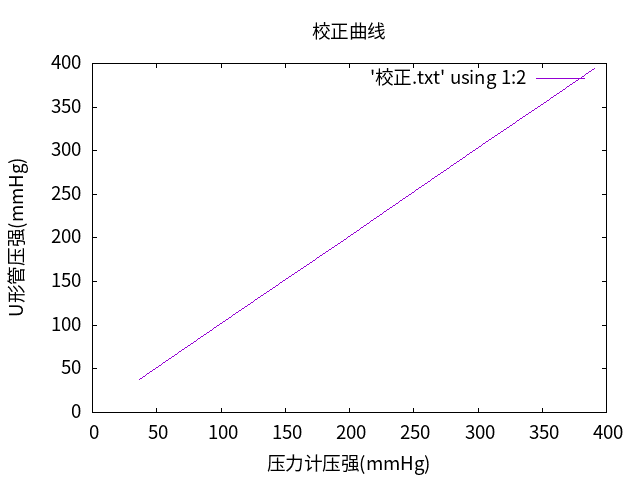
\includegraphics[width=.9\linewidth]{../img/校正.png}
\caption{校正曲线}
\end{figure}

\begin{verbatim}
iter      chisq       delta/lim  lambda   k             b            
   0 3.2330000000e+01   0.00e+00  1.70e+02    1.000000e+00   1.000000e+00
   1 4.5073306803e-01  -7.07e+06  1.70e+01    1.007076e+00   1.000023e+00
   2 3.7821603147e-01  -1.92e+04  1.70e+00    1.007431e+00   9.996930e-01
   3 3.7538416865e-01  -7.54e+02  1.70e-01    1.007500e+00   9.808530e-01
   4 3.7402735590e-01  -3.63e+02  1.70e-02    1.007591e+00   9.562873e-01
   5 3.7402712517e-01  -6.17e-02  1.70e-03    1.007592e+00   9.559628e-01
iter      chisq       delta/lim  lambda   k             b            

After 5 iterations the fit converged.
final sum of squares of residuals : 0.374027
rel. change during last iteration : -6.16862e-07

degrees of freedom    (FIT_NDF)                        : 8
rms of residuals      (FIT_STDFIT) = sqrt(WSSR/ndf)    : 0.216225
variance of residuals (reduced chisquare) = WSSR/ndf   : 0.0467534

Final set of parameters            Asymptotic Standard Error
=======================            ==========================
k               = 1.00759          +/- 0.0006073    (0.06027%)
b               = 0.955963         +/- 0.1461       (15.28%)

correlation matrix of the fit parameters:
#                k      b      
k               1.000 
b              -0.884  1.000 

\end{verbatim}

校正结果为
\[
    P_{Real}=P\times 1.00759+0.955963
    \]

\section{实验数据的校准绘图}
\label{sec:orgf058d2d}
利用之前得到的精确压强换算公式将数字压强计的读数换算成U形管压强计的读数,并将单位换算为Pa,
用外界大气压减去压差算出内部压强,
之后再将温度的单位换算为K,绘制p-T图
\begin{enumerate}
\item 第一组
\label{sec:org0f10777}
\begin{center}
\begin{tabular}{rrr}
序号 & 压强(Pa) & 温度(K)\\
\hline
1 & 98276.55 & 352.613\\
2 & 93372.95 & 350.939\\
3 & 87354.78 & 348.781\\
4 & 81968.56 & 346.756\\
5 & 76594.33 & 344.608\\
6 & 71314.77 & 342.392\\
7 & 66129.86 & 340.085\\
8 & 60810.30 & 337.550\\
9 & 55625.39 & 334.918\\
10 & 50425.82 & 332.078\\
\end{tabular}
\end{center}

数据绘图如下
\begin{figure}[htbp]
\centering
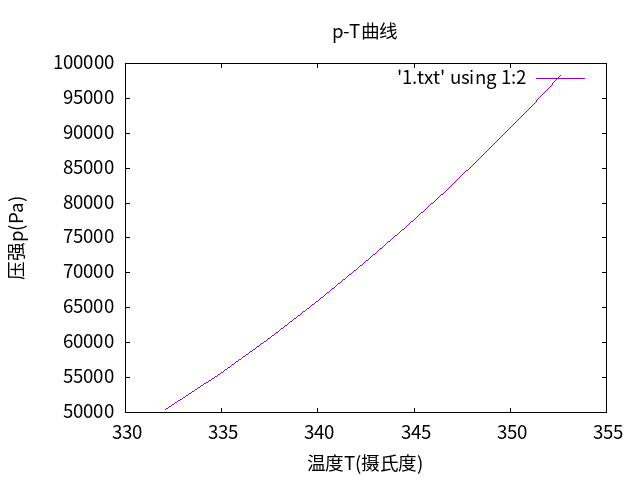
\includegraphics[width=.9\linewidth]{../data/1.png}
\caption{First-p-T}
\end{figure}

\item 第二组
\label{sec:org51ed222}
\begin{center}
\begin{tabular}{rrr}
序号 & 压强(Pa) & 温度(K)\\
\hline
1 & 50923.11 & 332.342\\
2 & 55464.07 & 334.826\\
3 & 60662.31 & 337.479\\
4 & 65941.88 & 339.996\\
5 & 71086.79 & 342.304\\
6 & 76125.04 & 344.429\\
7 & 81685.92 & 346.657\\
8 & 86629.51 & 348.536\\
9 & 91909.08 & 350.458\\
10 & 97160.64 & 352.284\\
\end{tabular}
\end{center}

数据绘图如下
\begin{figure}[htbp]
\centering
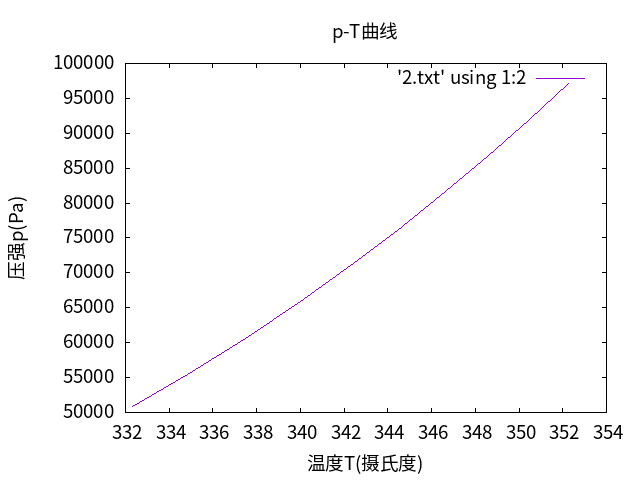
\includegraphics[width=.9\linewidth]{../data/2.png}
\caption{Second-p-T}
\end{figure}

\item 第三组
\label{sec:org42f22fb}
\begin{center}
\begin{tabular}{rrr}
序号 & 压强(Pa) & 温度(K)\\
\hline
1 & 97872.58 & 352.504\\
2 & 92875.66 & 350.788\\
3 & 87288.12 & 348.774\\
4 & 82021.89 & 346.750\\
5 & 76943.64 & 344.755\\
6 & 71798.73 & 342.594\\
7 & 66492.50 & 340.228\\
8 & 61119.61 & 337.689\\
9 & 55961.37 & 335.081\\
10 & 50332.49 & 331.990\\
\end{tabular}
\end{center}

数据绘图如下
\begin{figure}[htbp]
\centering
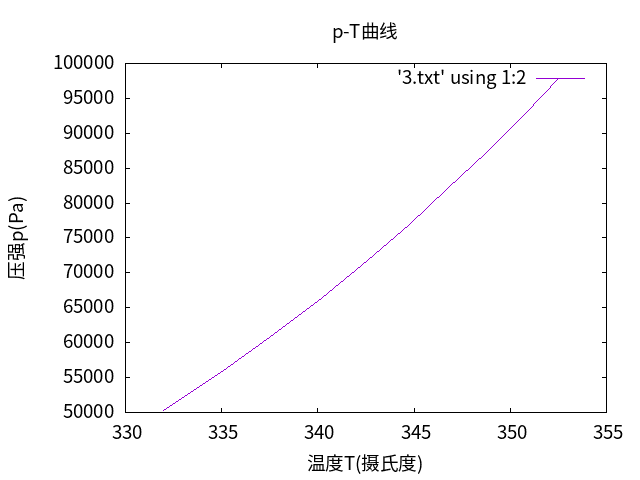
\includegraphics[width=.9\linewidth]{../data/3.png}
\caption{Third-p-T}
\end{figure}
\end{enumerate}
\section{线性拟合数据点}
\label{sec:orga3904b1}
利用\(\ln(p)\) 对\(1/T\) 作图, 根据拟合曲线的斜率求出摩尔汽化焓
\begin{enumerate}
\item 第一组(31880.864(J\(\cdot\) mol\textsuperscript{-1}))
\label{sec:orge73be4d}
\begin{center}
\begin{tabular}{rrrrr}
序号 & p(Pa) & T(K) & 1/T & ln(p)\\
\hline
1 & 98276.55 & 352.613 & 0.00284 & 11.496\\
2 & 93372.95 & 350.939 & 0.00285 & 11.444\\
3 & 87354.78 & 348.781 & 0.00287 & 11.378\\
4 & 81968.56 & 346.756 & 0.00288 & 11.314\\
5 & 76594.33 & 344.608 & 0.00290 & 11.246\\
6 & 71314.77 & 342.392 & 0.00292 & 11.175\\
7 & 66129.86 & 340.085 & 0.00294 & 11.099\\
8 & 60810.30 & 337.550 & 0.00296 & 11.016\\
9 & 55625.39 & 334.918 & 0.00299 & 10.926\\
10 & 50425.82 & 332.078 & 0.00301 & 10.828\\
\end{tabular}
\end{center}

数据绘图如下
\begin{figure}[htbp]
\centering
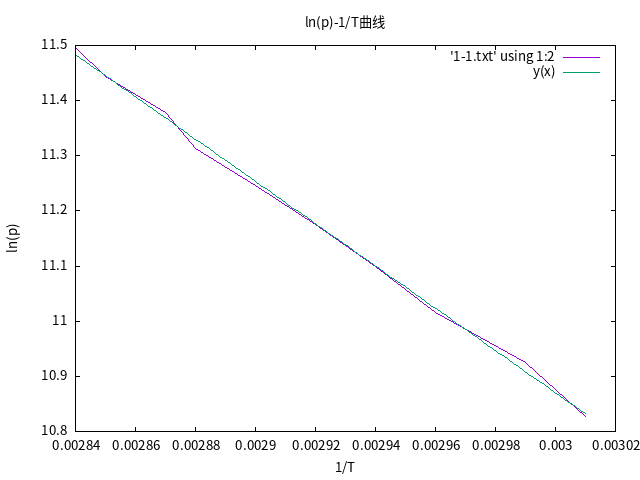
\includegraphics[width=.9\linewidth]{../data/1-1.png}
\caption{First-ln(p)-1/T}
\end{figure}

拟合结果如下
\begin{verbatim}
iter      chisq       delta/lim  lambda   k             b            
   0 1.0386668009e+03   0.00e+00  7.07e-01    1.000000e+00   1.000000e+00
   1 2.8059527571e+00  -3.69e+07  7.07e-02    1.028062e+00   1.070400e+01
   2 4.5171860642e-01  -5.21e+05  7.07e-03    1.005972e+00   1.118902e+01
   3 4.5116607068e-01  -1.22e+02  7.07e-04   -1.343005e+00   1.119612e+01
   4 4.0067523013e-01  -1.26e+04  7.07e-05   -2.226776e+02   1.184153e+01
   5 8.8149201195e-03  -4.45e+06  7.07e-06   -3.327865e+03   2.089626e+01
   6 9.4734986520e-04  -8.30e+05  7.07e-07   -3.833770e+03   2.237147e+01
   7 9.4732898172e-04  -2.20e+00  7.07e-08   -3.834595e+03   2.237388e+01
   8 9.4732898172e-04  -2.08e-09  7.07e-09   -3.834595e+03   2.237388e+01
iter      chisq       delta/lim  lambda   k             b            

After 8 iterations the fit converged.
final sum of squares of residuals : 0.000947329
rel. change during last iteration : -2.08296e-14

degrees of freedom    (FIT_NDF)                        : 8
rms of residuals      (FIT_STDFIT) = sqrt(WSSR/ndf)    : 0.0108819
variance of residuals (reduced chisquare) = WSSR/ndf   : 0.000118416

Final set of parameters            Asymptotic Standard Error
=======================            ==========================
k               = -3834.6          +/- 62.17        (1.621%)
b               = 22.3739          +/- 0.1813       (0.8104%)

correlation matrix of the fit parameters:
#                k      b      
k               1.000 
b              -1.000  1.000 

\end{verbatim}

直线的斜率为-3834.6,所以-B= -3834.6,B=3834.6,根据公式:
\[
     \Delta_{vap}H_{m}=RB
     \]
可计算得环己烷在58\textsuperscript{o}C\textasciitilde{}80\textsuperscript{o}C范围内的摩尔汽化热为:
\[
     \Delta_{vap}H_{m}=RB=8.314\times 3834.6=31880.864(J\cdot mol^{-1})
     \]
\item 第二组(31054.287(J\(\cdot\) mol\textsuperscript{-1}))
\label{sec:org29f005c}
\begin{center}
\begin{tabular}{rrrrr}
序号 & p(Pa) & T(K) & 1/T & ln(p)\\
\hline
1 & 50923.11 & 332.342 & 0.00301 & 10.838\\
2 & 55464.07 & 334.826 & 0.00299 & 10.923\\
3 & 60662.31 & 337.479 & 0.00296 & 11.013\\
4 & 65941.88 & 339.996 & 0.00294 & 11.097\\
5 & 71086.79 & 342.304 & 0.00292 & 11.172\\
6 & 76125.04 & 344.429 & 0.00290 & 11.240\\
7 & 81685.92 & 346.657 & 0.00288 & 11.311\\
8 & 86629.51 & 348.536 & 0.00287 & 11.369\\
9 & 91909.08 & 350.458 & 0.00285 & 11.429\\
10 & 97160.64 & 352.284 & 0.00284 & 11.484\\
\end{tabular}
\end{center}
数据绘图如下
\begin{figure}[htbp]
\centering
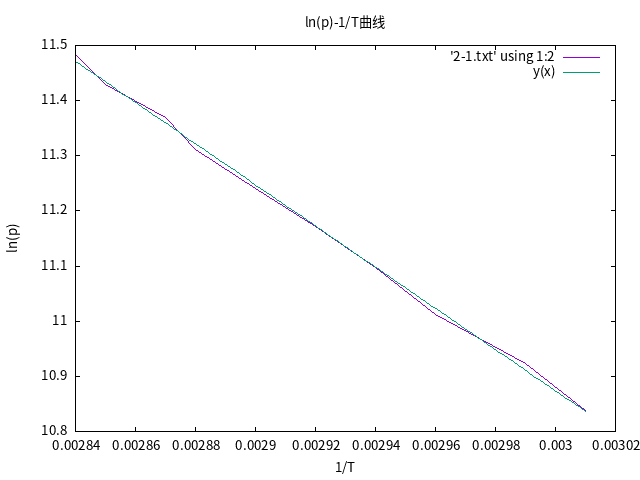
\includegraphics[width=.9\linewidth]{../data/2-1.png}
\caption{Second-ln(p)-1/T}
\end{figure}

拟合结果如下
\begin{verbatim}
iter      chisq       delta/lim  lambda   k             b            
   0 1.0377062871e+03   0.00e+00  7.07e-01    1.000000e+00   1.000000e+00
   1 2.7805161084e+00  -3.72e+07  7.07e-02    1.028055e+00   1.069962e+01
   2 4.2840741530e-01  -5.49e+05  7.07e-03    1.006574e+00   1.118442e+01
   3 4.2788312032e-01  -1.23e+02  7.07e-04   -1.281521e+00   1.119134e+01
   4 3.7997562692e-01  -1.26e+04  7.07e-05   -2.168795e+02   1.182002e+01
   5 8.1647213910e-03  -4.55e+06  7.07e-06   -3.241586e+03   2.064007e+01
   6 6.9969279148e-04  -1.07e+06  7.07e-07   -3.734379e+03   2.207705e+01
   7 6.9967297650e-04  -2.83e+00  7.07e-08   -3.735183e+03   2.207939e+01
   8 6.9967297650e-04  -6.29e-09  7.07e-09   -3.735183e+03   2.207939e+01
iter      chisq       delta/lim  lambda   k             b            

After 8 iterations the fit converged.
final sum of squares of residuals : 0.000699673
rel. change during last iteration : -6.29131e-14

degrees of freedom    (FIT_NDF)                        : 8
rms of residuals      (FIT_STDFIT) = sqrt(WSSR/ndf)    : 0.00935196
variance of residuals (reduced chisquare) = WSSR/ndf   : 8.74591e-05

Final set of parameters            Asymptotic Standard Error
=======================            ==========================
k               = -3735.18         +/- 53.43        (1.43%)
b               = 22.0794          +/- 0.1558       (0.7057%)

correlation matrix of the fit parameters:
#                k      b      
k               1.000 
b              -1.000  1.000 

\end{verbatim}
直线的斜率为-3735.18,所以-B= -3735.18,B=3735.18,根据公式:
\[
     \Delta_{vap}H_{m}=RB
     \]
可计算得环己烷在58\textsuperscript{o}C\textasciitilde{}80\textsuperscript{o}C范围内的摩尔汽化热为:
\[
     \Delta_{vap}H_{m}=RB=8.314\times 3735.18=31054.287(J\cdot mol^{-1})
     \]
\item 第三组(32285.341(J\(\cdot\) mol\textsuperscript{-1}))
\label{sec:orgd7bee62}
\begin{center}
\begin{tabular}{rrrrr}
序号 & p(Pa) & T(K) & 1/T & ln(p)\\
\hline
1 & 97872.58 & 352.504 & 0.00284 & 11.491\\
2 & 92875.66 & 350.788 & 0.00285 & 11.439\\
3 & 87288.12 & 348.774 & 0.00287 & 11.377\\
4 & 82021.89 & 346.750 & 0.00288 & 11.315\\
5 & 76943.64 & 344.755 & 0.00290 & 11.251\\
6 & 71798.73 & 342.594 & 0.00292 & 11.182\\
7 & 66492.50 & 340.228 & 0.00294 & 11.105\\
8 & 61119.61 & 337.689 & 0.00296 & 11.021\\
9 & 55961.37 & 335.081 & 0.00298 & 10.932\\
10 & 50332.49 & 331.990 & 0.00301 & 10.826\\
\end{tabular}
\end{center}
数据绘图如下
\begin{figure}[htbp]
\centering
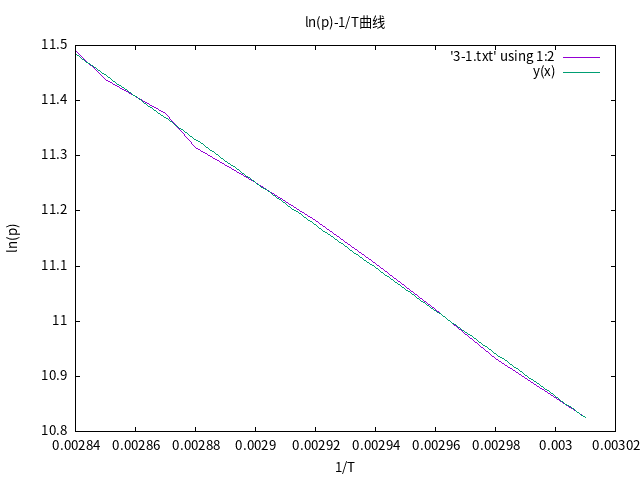
\includegraphics[width=.9\linewidth]{../data/3-1.png}
\caption{Third-ln(p)-1/T}
\end{figure}

拟合结果如下
\begin{verbatim}
iter      chisq       delta/lim  lambda   k             b            
   0 1.0390036548e+03   0.00e+00  7.07e-01    1.000000e+00   1.000000e+00
   1 2.7969241079e+00  -3.70e+07  7.07e-02    1.028065e+00   1.070562e+01
   2 4.4190422274e-01  -5.33e+05  7.07e-03    1.006756e+00   1.119072e+01
   3 4.4138776635e-01  -1.17e+02  7.07e-04   -1.264165e+00   1.119759e+01
   4 3.9401251558e-01  -1.20e+04  7.07e-05   -2.158059e+02   1.182297e+01
   5 8.9808202758e-03  -4.29e+06  7.07e-06   -3.347847e+03   2.095287e+01
   6 5.9621587061e-04  -1.41e+06  7.07e-07   -3.882334e+03   2.251090e+01
   7 5.9619145299e-04  -4.10e+00  7.07e-08   -3.883248e+03   2.251357e+01
   8 5.9619145299e-04  -4.98e-09  7.07e-09   -3.883248e+03   2.251357e+01
iter      chisq       delta/lim  lambda   k             b            

After 8 iterations the fit converged.
final sum of squares of residuals : 0.000596191
rel. change during last iteration : -4.98282e-14

degrees of freedom    (FIT_NDF)                        : 8
rms of residuals      (FIT_STDFIT) = sqrt(WSSR/ndf)    : 0.00863272
variance of residuals (reduced chisquare) = WSSR/ndf   : 7.45239e-05

Final set of parameters            Asymptotic Standard Error
=======================            ==========================
k               = -3883.25         +/- 50.48        (1.3%)
b               = 22.5136          +/- 0.1472       (0.6537%)

correlation matrix of the fit parameters:
#                k      b      
k               1.000 
b              -1.000  1.000 

\end{verbatim}
直线的斜率为-3883.25,所以-B=-3883.25,B=3883.25,根据公式:
\[
     \Delta_{vap}H_{m}=RB
     \]
可计算得环己烷在58\textsuperscript{o}C\textasciitilde{}80\textsuperscript{o}C范围内的摩尔汽化热为:
\[
     \Delta_{vap}H_{m}=RB=8.314\times 3883.25=32285.341(J\cdot mol^{-1})
     \]
\end{enumerate}

\section{计算平均摩尔汽化热}
\label{sec:orgf75faeb}
\[
    \overline{\Delta_{vap}H_{m}}=\frac{\Delta_{vap}H_{m1}+\Delta_{vap}H_{m2}+\Delta_{vap}H_{m3}}{3}
    \]
\[
    \overline{\Delta_{vap}H_{m}}=(31880.864+31054.287+32285.341)/3=31740.164(J\cdot mol^{-1})
    \]
经百度得知环己烷的摩尔汽化热为31.51 kJ/mol(不同资料给出的结果不同),所以两者的相对误差为:
\[
    w=\frac{31740.164-31510}{31510}\times 100\% =0.73\%
    \]
由上述相对误差可知,实验所测的平均摩尔汽化热与理论摩尔汽化热相差较小,说明实验结果的准确性。
\section{由曲线求得待测液体的正常沸点,并与文献值比较}
\label{sec:org99f64d5}
\begin{enumerate}
\item 第一组(353.49(K))
\label{sec:org68014ba}
\begin{itemize}
\item k= -3834.6
\item b= 22.3739
\end{itemize}
拟合曲线为:
\[
     \ln(p)=-\frac{3834.6}{T}+22.3739
     \]
所以当压力为大气压即P=101325Pa时,温度即沸点为:
\[
     T=-\frac{3834.6}{\ln(101325)-22.3739}=353.49(K)
     \]
\item 第二组(353.93(K))
\label{sec:orga9d3cad}
\begin{itemize}
\item k= -3735.18
\item b= 22.0794
\end{itemize}
拟合曲线为:
\[
     \ln(p)=-\frac{3735.18}{T}+22.0794
     \]
所以当压力为大气压即P=101325Pa时,温度即沸点为:
\[
     T=-\frac{3735.18}{\ln(101325)-22.0794}=353.93(K)
     \]
\item 第三组(353.42(K))
\label{sec:org5fbba76}
\begin{itemize}
\item k= -3883.25
\item b= 22.5136
\end{itemize}
拟合曲线为:
\[
     \ln(p)=-\frac{3883.25}{T}+22.5136
     \]
所以当压力为大气压即P=101325Pa时,温度即沸点为:
\[
     T=-\frac{3883.25}{\ln(101325)-22.5136}=353.42(K)
     \]
\item 误差分析
\label{sec:orgdd8df57}
查得(经百度百科)环己烷在大气压下的理论沸点为80.7\textsuperscript{o}C,即353.85K,与实验所测的沸点进行比较可知,
绝对误差及相对误差分别为:
\begin{enumerate}
\item 第一组
\label{sec:orgf5e87ae}
\[
      \Delta T=353.49-353.85=-0.36(K)
      \]
\[
      w=\frac{|\Delta T|}{T}=\frac{0.36}{353.85}=0.10\%
      \]
\item 第二组
\label{sec:org7b9eba0}
\[
      \Delta T=353.93-353.85=0.08(K)
      \]
\[
      w=\frac{|\Delta T|}{T}=\frac{0.08}{353.85}=0.02\%
      \]
\item 第三组
\label{sec:orgcbb65f0}
\[
      \Delta T=353.42-353.85=0.43(K)
      \]
\[
      w=\frac{|\Delta T|}{T}=\frac{0.43}{353.85}=0.12\%
      \]
\item 结论
\label{sec:orgc3fe4b5}
由上述相对误差可知,实验所测的正常沸点与理论值偏差较小,
说明实验结果较为准确,实验方法较为合理。
\end{enumerate}
\end{enumerate}
\end{document}
